\documentclass[tikz, border=2mm]{standalone}
\begin{document}

% 1. subset-intersection.png
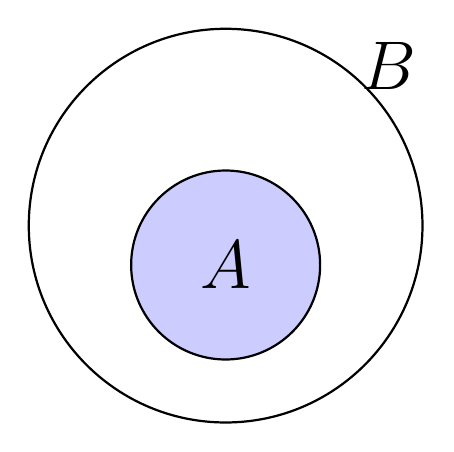
\begin{tikzpicture}
    % A inside B
    \fill[blue!20] (0,-0.5) circle (1.2cm);
    \draw[thick] (0,0) circle (2.5cm) node[above right=1.6cm] {\Huge $B$};
    \draw[thick] (0,-0.5) circle (1.2cm) node {\Huge $A$};
\end{tikzpicture}

% 2. commutative-intersection.png
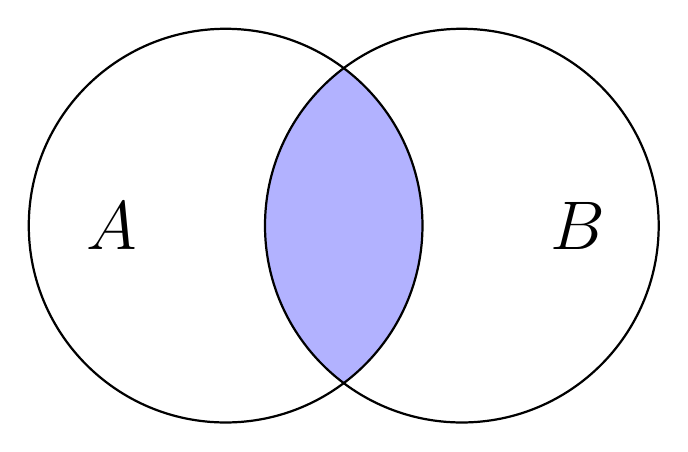
\begin{tikzpicture}
    \begin{scope}
        \clip (-1.5,0) circle (2.5cm);
        \fill[blue!30] (1.5,0) circle (2.5cm);
    \end{scope}
    \draw[thick] (-1.5,0) circle (2.5cm) node[left=1cm] {\Huge $A$};
    \draw[thick] (1.5,0) circle (2.5cm) node[right=1cm] {\Huge $B$};
\end{tikzpicture}

% 3. commutative-union.png
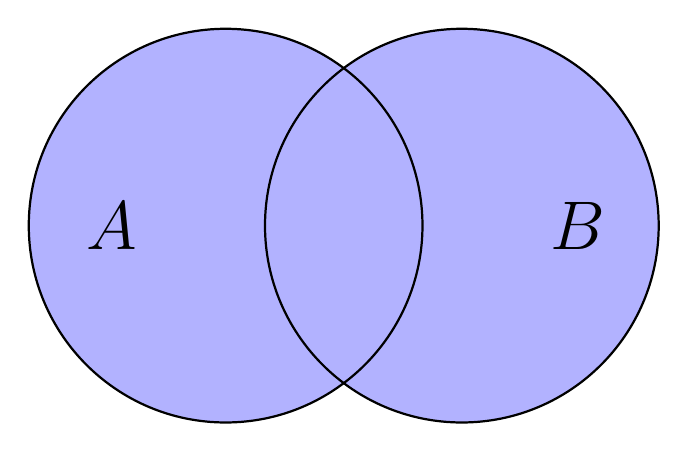
\begin{tikzpicture}
    \fill[blue!30] (-1.5,0) circle (2.5cm);
    \fill[blue!30] (1.5,0) circle (2.5cm);
    \draw[thick] (-1.5,0) circle (2.5cm) node[left=1cm] {\Huge $A$};
    \draw[thick] (1.5,0) circle (2.5cm) node[right=1cm] {\Huge $B$};
\end{tikzpicture}

% 4. associative-union.png
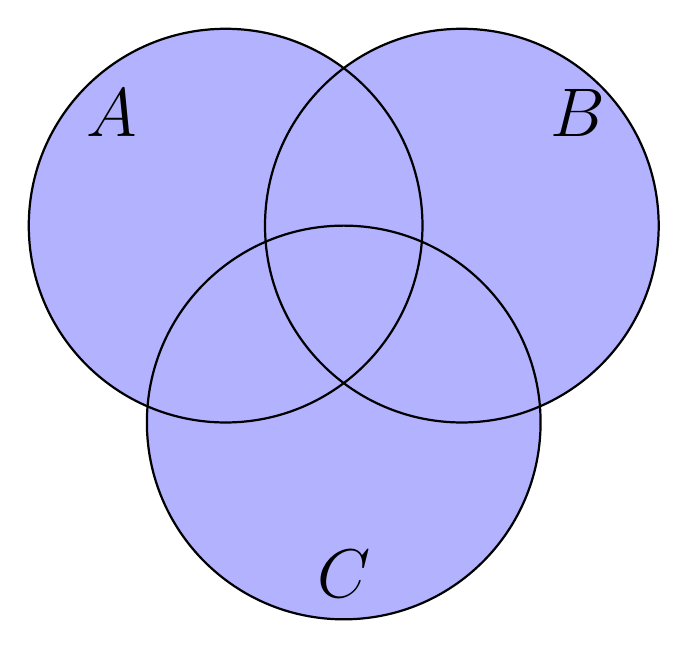
\begin{tikzpicture}
    \fill[blue!30] (-1.5,1) circle (2.5cm);
    \fill[blue!30] (1.5,1) circle (2.5cm);
    \fill[blue!30] (0,-1.5) circle (2.5cm);
    
    \draw[thick] (-1.5,1) circle (2.5cm) node[above left=1cm] {\Huge $A$};
    \draw[thick] (1.5,1) circle (2.5cm) node[above right=1cm] {\Huge $B$};
    \draw[thick] (0,-1.5) circle (2.5cm) node[below=1.5cm] {\Huge $C$};
\end{tikzpicture}

% 5. associative-intersection.png
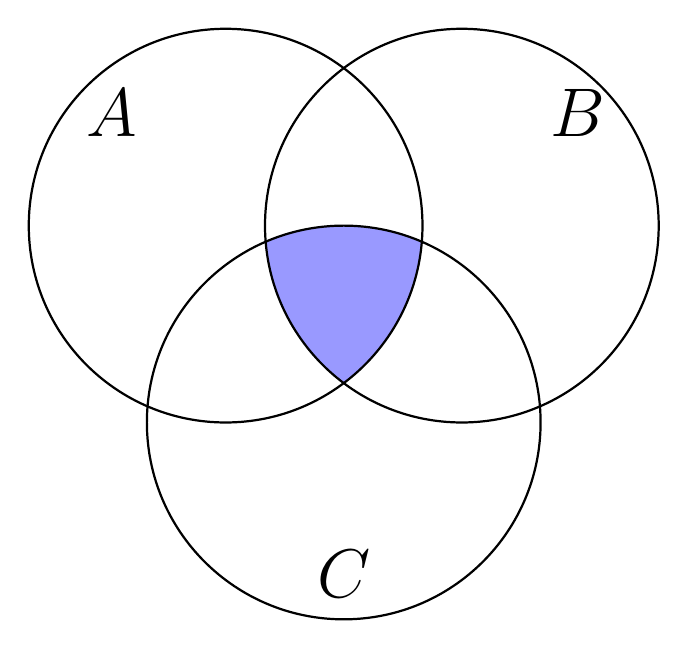
\begin{tikzpicture}
    \begin{scope}
        \clip (-1.5,1) circle (2.5cm);
        \clip (1.5,1) circle (2.5cm);
        \fill[blue!40] (0,-1.5) circle (2.5cm);
    \end{scope}
    
    \draw[thick] (-1.5,1) circle (2.5cm) node[above left=1cm] {\Huge $A$};
    \draw[thick] (1.5,1) circle (2.5cm) node[above right=1cm] {\Huge $B$};
    \draw[thick] (0,-1.5) circle (2.5cm) node[below=1.5cm] {\Huge $C$};
\end{tikzpicture}

\end{document}
